\documentclass[11pt]{article}

% ==== Paquetes ====
\usepackage[utf8]{inputenc}
\usepackage[T1]{fontenc}
\usepackage[spanish]{babel}
\usepackage{amsmath, amssymb, amsfonts}
\usepackage{graphicx}
\usepackage{caption}
\usepackage{subcaption}
\usepackage{float}
\usepackage{geometry}
\usepackage{hyperref}
\usepackage{minted}
\usepackage{mdframed}
\geometry{margin=2.3cm}

\usemintedstyle{friendly}
\setminted{fontsize=\scriptsize, breaklines=true}

% ==== Datos de la tarea ====
\title{IEE3864 – Fundamentos de instrumentación astronómica \\ \large Tarea 5}
\author{Nicolás Seguel}
\date{\today}

\begin{document}
\maketitle

\begin{enumerate}
    \item \textbf{Derive an expression for the angular magnification provided by the Galilean and Keplerian telescopes as function of the parameters of the telescopes, i.e. the focals of the lenses used.}
    
\begin{figure}[H]
    \centering
    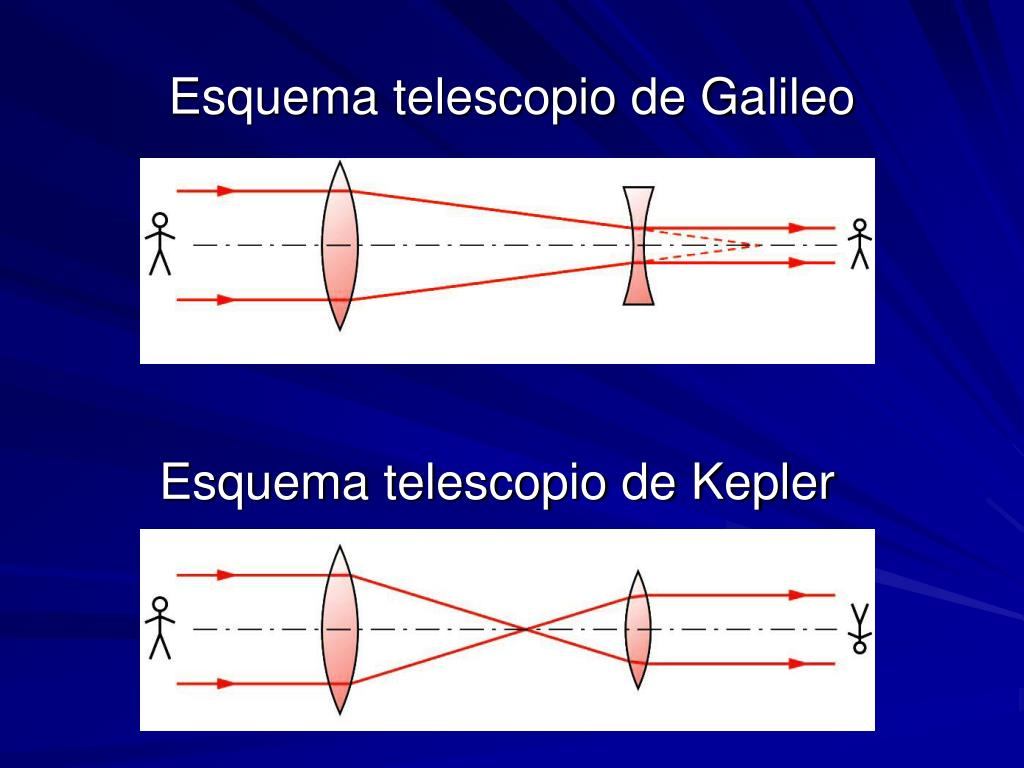
\includegraphics[width=0.8\textwidth]{galileo_kepler.jpg}
    \caption{Esquema de los telescopios Galileo y Kepler.}
    \label{fig:telescopes}
\end{figure}

En un telescopio Galileo, la lente objetivo es convergente y la lente ocular es divergente. Usando matrices de trasferencia óptica, tenemos:

\[
\begin{bmatrix}1 & 0 \\
\frac{1}{f_2} & 1\end{bmatrix}
\begin{bmatrix}1 & d \\
0 & 1\end{bmatrix}
\begin{bmatrix}1 & 0 \\
-\frac{1}{f_1} & 1\end{bmatrix}
\]

Resolviendo esta multiplicación se tiene:

\[
\begin{bmatrix}\frac{f_2}{f_1} & f_1 - f_2 \\
0 & \frac{f_1}{f_2}\end{bmatrix}
\]

Asumiendo que \(\theta = 0\), la magnificación angular es:

\[M = \frac{f_1}{f_2}\]

Para el telescopio Kepler, ambas lentes son convergentes. Usando el mismo procedimiento, tenemos: 

\[
\begin{bmatrix}1 & 0 \\
-\frac{1}{f_2} & 1\end{bmatrix}
\begin{bmatrix}1 & f_1 + f_2 \\
0 & 1\end{bmatrix}
\begin{bmatrix}1 & 0 \\
-\frac{1}{f_1} & 1\end{bmatrix}
\]

Resolviendo esta multiplicación se tiene:

\[
\begin{bmatrix}-\frac{f_2}{f_1} & f_1 + f_2 \\
0 & -\frac{f_1}{f_2}\end{bmatrix}
\]

Asumiendo que \(\theta = 0\), la magnificación angular es:

\[M = -\frac{f_1}{f_2}\]


    \item \textbf{Derive an expression for the effective focal length (EFL) of a system formed by two lenses (or two mirrors) as function of the focals of the lenses and their distances: f1, f2 and d. Fig. 5.2}
    
La distancia focal efectiva (EFL) corresponde a la distancia focal de un lente o espejo que produce el mismo efecto que el sistema real. Para un sistema de dos lentes, la fórmula para calcular la EFL es:

\[\frac{1}{EFL} = \frac{1}{f_1} + \frac{1}{f_2} - \frac{d}{f_1 f_2}\]

    \item \textbf{Calculate BFL and EFL of the combination of two spherical mirrors shown in the class. Fig. 5.3}


\end{enumerate}

\end{document}